%! TEX root = 'main.tex'
\section{Experiment}
\label{sec:experiment}

\subsection{Reverse Engineering}
The PLC we use in this paper is Allen-Bradley 1769-L18ER-BB1B/B CompactLogix 5370. The reverse engineering process consists of two parts. The hardware part is primarily wire tracing, and the software part is to analyze the disassembly of the dumped firmware.

First, we need to determine each module in the PLC and check the microcontroller model and other essential IC chips. Next, we need to dump the firmware from the microcontroller and other chips.

\textbf{\textit{Backplanes.}} The Allen-Bradley CompactLogix 5370 contains several PCB module boards, known as backplanes. ~\autoref{fig:modules} shows that it contains one communication module, one real-time controller module, DC digital input/output module, and the power supply module. They are interconnected through proPrutoref{tab:memorymap} shows the memory map.ietary sockets.

The communication module \textbf{B} itself is a complete embedded system, including a CPU, DRAM, and other peripherals such as ethernet, SD card socket, and USB port. Its function is to communicate with the host to update firmware and ladder logic, and it also contains a web server. On the one hand, this module is not the one that controls IO, not our target. On the other hand, two FPGA chips are used to implement the processor and other peripheral devices such as the ethernet controller, making it very difficult to find the JTAG interface.

We focus on the real-time controller, which mainly executes the compiled ladder logic and controls the IO accordingly. Fortunately, the module uses a commercial microcontroller, Stellaris LM3S2793 SoC from Texas Instruments.

The IO module \textbf{D} has 16 inputs and 16 outputs socket, connecting to the real-time module \textbf{B}, through power switch and optically coupled isolator chips, eventually connected to the pins of the microcontroller. The LED module \textbf{E} contains LED lights for each IO socket and the status indicator of the PLC. Its wire goes through the communication module's PCB board and connects to the real-time module. Instead of directly connects each LED light, the microcontroller controls the LED module through the I2C protocol. The power module \textbf{A} provides stable 3 volts for other boards. The backdoor implant can either get power directly from it or the JTAG pad on the real-time module.

\begin{figure}[th]
	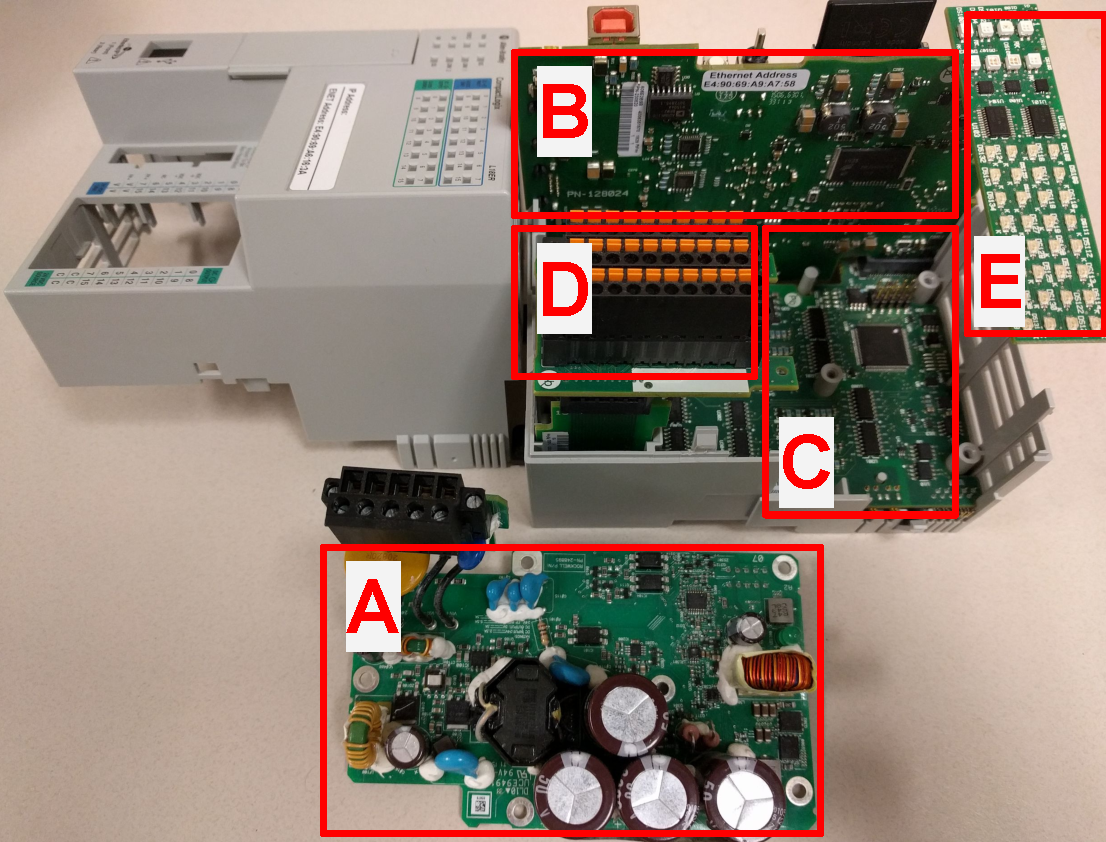
\includegraphics[width=0.47\textwidth]{figures/modules}
	\centering
	\caption{Allen-Bradley 1769-L18ER-BB1B/B CompactLogix 5370 PLC. A: Power supply module  B: Communication module  C: Real-time module  D: (16) DC Digital Outputs \& (16) DC Digital Inputs  E: LED indicator module}
	\label{fig:modules}
\end{figure}




\textbf{\textit{Microcontroller.}} The TI Stellaris LM3S2793 SoC has an ARM Cortex-M3 processor core that operates at 80 MHz. It contains 64 KB SRAM and 128 KB flash. The internal ROM is preprogrammed with Stellaris Peripheral Driver Library (DriverLib) to drive the on-chip peripheral devices. ~\autoref{tab:memorymap} shows the memory map. 


\begin{center}
	\begin{table}
		\begin{tabular}{|p{1.6cm} p{1.6cm} p{4cm}|} 
			\hline
			Start & End & Description \\ [0.5ex] 
			\hline
			0x00000000 & 0x0001FFFF & On-chip Flash \\ 
			\hline
			0x00020000 & 0x00FFFFFF & Reserved \\
			\hline
			0x01000000 & 0x1FFFFFFF & Reserved for ROM \\
			\hline
			0x20000000 & 0x2000FFFF & Bit-banded on-chip SRAM \\
			\hline
			0x20010000 & 0x21FFFFFF & Reserved \\
			\hline
			0x22000000 & 0x221FFFFF & Bit-band alias of bit-banded on-chip SRAM starting at 0x20000000 \\
			\hline
			0x22200000 & 0x3FFFFFFF & Reserved \\
			\hline
		\end{tabular}
		\caption{LM3S2793 Memory Map}
		\label{tab:memorymap}
	\end{table}
\end{center}



\textbf{\textit{Reset Vector.}} The vector table is fixed at address 0x00000000 on system reset. Once a core is out of reset sequence, it starts executing from memory address 0x00000004, the reset vector.  From the memory map, the reset vector resides in the flash memory instead of the ROM. The reason is that the ROM boot loader is only used as an initial program loader when the flash memory is empty and as an application-initiated firmware upgrade mechanism. For instance, if the data at address 0x00000004 is 0xFFFFFFFF, the ROM is mapped to address 0x00000000, and execution continues out of the ROM boot loader. If there is data at address 0x00000004 that is not 0xFFFFFFFF, the stack pointer (SP) is loaded from Flash memory at address 0x00000000 and the program counter (PC) is loaded from address 0x00000004. The firmware then begins executing from the flash memory.


In our case, the SP value is 0x20000B48, and the PC is 0x000000E3. Notice that 0xE3 is an odd number, ARM is a RISC architecture that uses a fixed-length instruction encoding format which uses four bytes instruction for the 32-bit processor. Certainly, the least significant bit indicates that the next branch uses Thumb instructions. Therefore we dump the flash memory and start to disassemble at address 0x000000E2.

\textbf{\textit{Flash boot loader.}} The SRAM is at 0x20000000. The flash boot loader copies itself to SRAM memory right after it starts, in consideration of performance. Even though the SRAM and flash memory can both be accessed in a single cycle, the manual says that the flash memory only can do that as long as the code is linear and branches incur a one-cycle stall. 

The code copies memory range 0x0 - 0xA88 to 0x20000000 - 0x20000A88 and initialize the data section 0x20000A88 - 0x20000F54 to 0.  Next, it uses the vector table that resides in SRAM. As mentioned above, on system reset, the vector table is fixed at address 0x00000000. The privileged code can write to the Vector Table Offset (VTABLE) register to relocate the vector table start address to a different memory location aligned on a 512-byte boundary. Replacing the vector table could mean completely changing the system's behavior because the corresponding interrupt vectors will point to different interrupt handlers to process peripheral devices' requests.


Finally, it sets the vector table to 0x20000000 and jumps to SRAM to continue.



\textbf{\textit{Stellaris Peripheral Driver Library.}} The Drivelib~\cite{lm3s2793rom} uses tables to provide library API entries. The tables have two levels. The main table contains one pointer per peripheral, which points to a secondary table containing one pointer per API associated with that peripheral. The main table is located at 0x01000010, right after the Cortex-M3 vector table in the ROM. \autoref{tab:romtable} shows a portion of the API table, and ~\autoref{tab:gpiotable} shows part of the ROM\_GPIOTABLE, which contains the entry points of all the GPIO related APIs.

\begin{center}
	\begin{table}
		\small
		\begin{tabular}{|p{7.2cm}|} 
			\hline
			ROM\_APITABLE (0x1000010) \\ [0.5ex] 
			\hline
			[0] = ROM\_VERSION \\
			\hline
			[1] = pointer to ROM\_UARTTABLE \\
			\hline
			[2] = pointer to ROM\_SSITABLE \\
			\hline
			[3] = pointer to ROM\_I2CTABLE \\
			\hline
			[4] = pointer to ROM\_GPIOTABLE \\
			\hline
			[5] = pointer to ROM\_ADCTABLE \\
			\hline
			... \\ 
			\hline
		\end{tabular}
		\caption{LM3S2793 ROM API Table}
		\label{tab:romtable}
	\end{table}
\end{center}

\begin{center}
	\begin{table}
		\small
		\begin{tabular}{|p{7.2cm}|} 
			\hline
			ROM\_GPIOTABLE \\ [0.5ex] 
			\hline
			[0] = function ROM\_GPIOPinWrite \\
			\hline
			[1] = function ROM\_GPIODirModeSet \\
			\hline
			[2] = function ROM\_GPIODirModeGet \\
			\hline
			[3] = function ROM\_GPIOIntTypeSet \\
			\hline
			[4] = function ROM\_GPIOIntTypeGet \\
			\hline
%			[5] = function ROM\_GPIOPadConfigSet \\
%			\hline
			... \\ 
			\hline
		\end{tabular}
		\caption{GPIO API Table}
		\label{tab:gpiotable}
	\end{table}
\end{center}


%The following is an example of calling function ROM\_GPIOPinRead() from the flash memory disassembly. API table indexing 0x1000010 + 0x10 (ROM\_APITABLE[4]) is optimized to 0x1000020 which points to the GPIO API table. [R2,\#0x2C] represents ROM\_GPIOTABLE[11] which is ROM\_GPIOPinRead(). So the code that calling the ROM library is very helpful to reveal the intent of the program.


\autoref{fig:romapiexample} shows a typical code snippet calling a ROM API. The table is at 0x1000010 + 0x10 (ROM\_APITABLE[4]), the GPIO table and the API is ROM\_GPIOPinRead() (ROM\_GPIOTABLE[11]). All the ROM API call sites have the same pattern, which makes reverse engineering the firmware much easier.  Calling the ROM API is merely to find the function address from the two-level tables and then jump to it. There is no privilege change; all the code runs in the system mode.


\begin{figure}[th]
	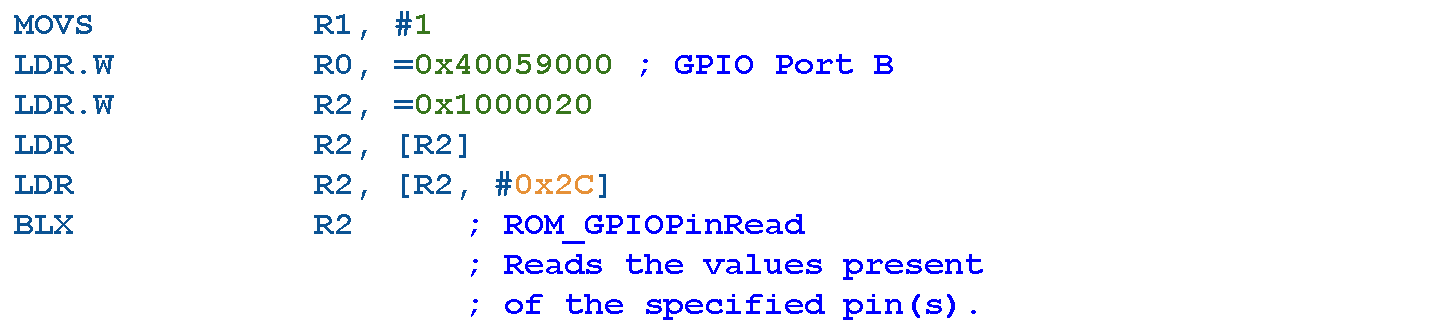
\includegraphics[width=0.47\textwidth]{figures/romapiexample2}
	\centering
	\caption{A code snippet calling ROM\_GPIOPinRead(). The parameters are passed in through the general registers where, in this case, the function has two parameters: R0 contains the GPIO port address to operate, and R1 is the bit-packed representation of the pins.  R2 stores the GPIO API table's address and eventually loads the API entry point and then jump to it.}
	\label{fig:romapiexample}
\end{figure}




\textbf{\textit{Debug.}} In addition to reverse-engineering,  we also need to debug the firmware. We use the SEGGER J-Link debugger. Since the target is ARM and the debugger sets up a GDB server, we also need GNU Embedded Toolchain for ARM~\cite{gnutoolchainarm}, an ARM version of the gdb client.


As mentioned earlier, the stack pointer and program counter are located at address 0x00000000 and 0x00000004. As shown in~\autoref{fig:gdbinit}, we use a GDB initialization script that contains GDB commands to set up the target. This script makes the PLC initialized and runs ladder logic, but the PLC cannot be interrupted during runtime with the debugger. If so, the indicator on the LED panel will prompt an IO error. The reason is still under investigation, and it could be that the watchdog timer is not handled well.

\begin{figure}[th]
	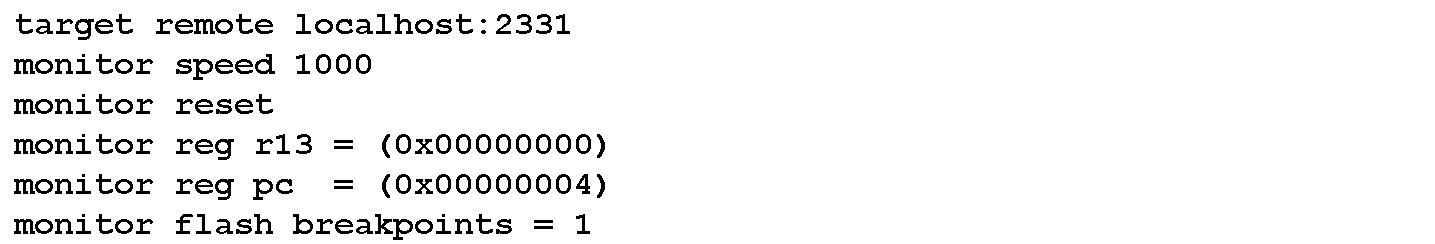
\includegraphics[width=0.47\textwidth]{figures/gdbinit}
	\centering
	\caption{The minimal gdbinit script that sets the SP and PC registers makes the PLC be up and running. Other on-chip peripheral controllers may not be correctly initialized.}
	\label{fig:gdbinit}
\end{figure}



%\subsubsection{more reverse engineering topics ....}

%Through reverse engineering, it shows that the Vector Table Offset Register is first at address 0x0, then switch to address 0x20000000, after receiving the ladder logic code, finally set to address 0x40000. 


\subsection{GPIO}

The hardware backdoor's essential function is to control the PLC's output to control the industrial physical system. The GPIO pins on the microcontroller either sensing the inputs or controls the outputs of the PLC.

For our target LM3S2793, the GPIO module comprises nine physical GPIO blocks, each corresponding to an individual GPIO port. Depending on the microcontroller's configuration, it supports up to 67 programmable input/output pins or several GPIOs grouped compose of a peripheral function such as I2C, and the GPIO ports can be accessed either through AHB or APB bus.  Each GPIO port has several associated control registers, such as GPIO Digital Enable (GPIODEN), GPIO Alternate Function Select (GPIOAFSEL), GPIO Port Control (GPIOPCTL), and GPIO Data Control registers. All GPIO pins are configured as GPIOs and tri-stated by default.

We primarily operate on the GPIO Data control registers. The GPIO Direction (GPIODIR) register configures each pin as an input or output, which should not be changed for the PLC's IO. The GPIO Data (GPIODATA) register modifies individual bits in GPIO ports. Different microcontrollers have their own operating methods on GPIOs, such as Output Data Register (ODR), Bit Reset Register (BRR), Bit Set/Reset Register (BSRR)~\cite{cottle2001programmable}. On LM3S2793, to modify individual GPIO pins in a single instruction without affecting the other pins' state, the operation on GPIODATA is not intuitive. Instead of each bit representing a GPIO pin,  it uses bits [9:2] of the address as a mask. Bits[1:0] are always zero because the memory access should be at 4-byte alignment on ARM.  For each GPIO port, it needs the memory range from GPIODATA to GPIODATA + 0x3FC to operate. If the address bit associated with that data bit is set during a write, the GPIODATA register's bit is altered. If the address bit is cleared, then the data bit is left unchanged.

For example, GPIO Port A (AHB) is at 0x40058000, and we want to set its bit-2 to 0 and bit-5 to 1. As shown in~\autoref{gpiowrite}, the address mask is 0x90, and the value we write is 0xF0.  Therefore, we need to write a value of 0xF0 to the address 0x40058090.

\begin{figure}[th]
	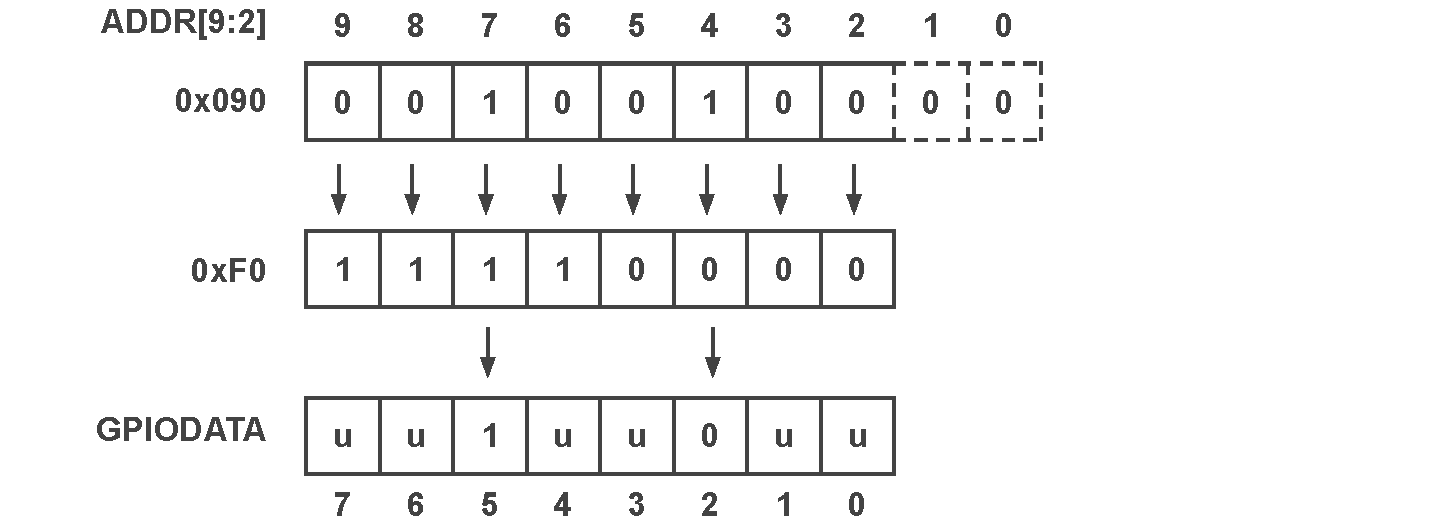
\includegraphics[width=0.47\textwidth]{figures/gpiowrite2}
	\centering
	\caption{GPIODATA Write Example. Writing a value of 0xF0 to the address GPIODATA + 0x090 has the bit-2 unset and bit-5 set in GPIODATA register where \textbf{u} indicates that data is unchanged by the write. Because of the mask, for example, writing 0xF0 or writing 0x2B has the same effect.}
	\label{fig:gpiowrite}
\end{figure}



To read a GPIO port, if the address bit associated with the data bit is set, the value is read. If the address bit associated with the data bit is cleared, the data bit is read as a zero, regardless of its actual value. For instance, we read GPIO Port A's high 4 bits. As shown in~\autoref{fig:gpioread}, the address mask is 0x3C0, and read address 0x400583C0 yields 0xA0.


\begin{figure}[th]
	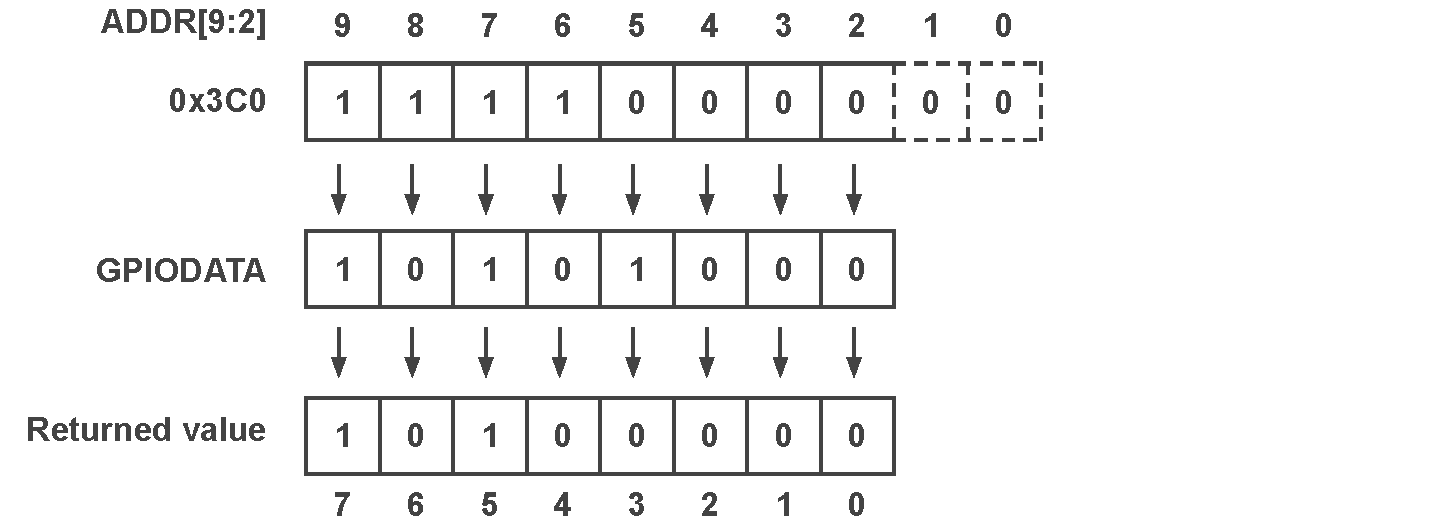
\includegraphics[width=0.47\textwidth]{figures/gpioread2}
	\centering
	\caption{GPIODATA Read Example. Reading address GPIODATA+0x3C0 returns the high 4 bits of the GPIO port because the address mask for the low 4 bits is all zeros.}
	\label{fig:gpioread}
\end{figure}



\subsection{Attacks}
After controlling JTAG, there are many ways to attack. One of the attacks is to change the IO output without changing the panel LED indicator and monitoring system. Through reverse engineering, we know that GPIO port E (0x4005C000), GPIO port F (0x4005D000) corresponds to IO inputs, and GPIO port G (0x4005E000), GPIO port H (0x4005F000) corresponds to IO outputs. Each GPIO port contains 8 effective bits, corresponding to each pin on the panel. As mentioned earlier, we can change the GPIO output by changing the GPIO Data (GPIODATA) register. For instance, to modify all the pins on GPIO port G, write a byte to address 0x4005E3FC. For each bit in the byte, zero means output field power voltage, 1 means output low voltage (8v).

The scan cycle is the cycle of which the PLC gathers the inputs, runs the ladder logic and then updates the outputs. Scan cycles repeat in milliseconds. It will update the outputs based on the ladder logic, here ladder logic refers to variables in memory. With some reverse engineering work, we can modify those variables accordingly to get the IO output we want. We also found an particular variable that controls the update of IO output. For example, this variable in our case is located at 0x20002D0B, it varies due to different firmware version. When this variable is set to 0, the IO module stops at the current state. So now we can change the output arbitrarily. After changing this variable back to the original value, everything is restored to the state corresponding to the ladder logic. So we have a time window of arbitrary length for malicious output. 



\subsection{Onboard Components Interconnection}
Knowing how the real-time controller controls IO module, how to attack attack through the JTAG interface, we hope to learn more about the other chips on the board and how the different backplanes are related. We found that no other chips are daisy chained together with LM3S2793 via JTAG, so we need more reverse engineering work.

\subsubsection{AT45DB021E SPI Serial Flash Memory}
Right next to the LM3S2793 microcontroller, there is a flash chip, "adesto 45DB021E SHN" printed on it. It's a 2-Mbit SPI serial flash memory chip. According to the pin diagram of the LM3S2793 and AT45DB021E and the multimeter connectivity test, we found that the flash chip is connected to the SSI0 (Synchronous Serial Interface) of LM3S2793 as shown in~\autoref{fig:ssi0}.

\begin{figure}[th]
	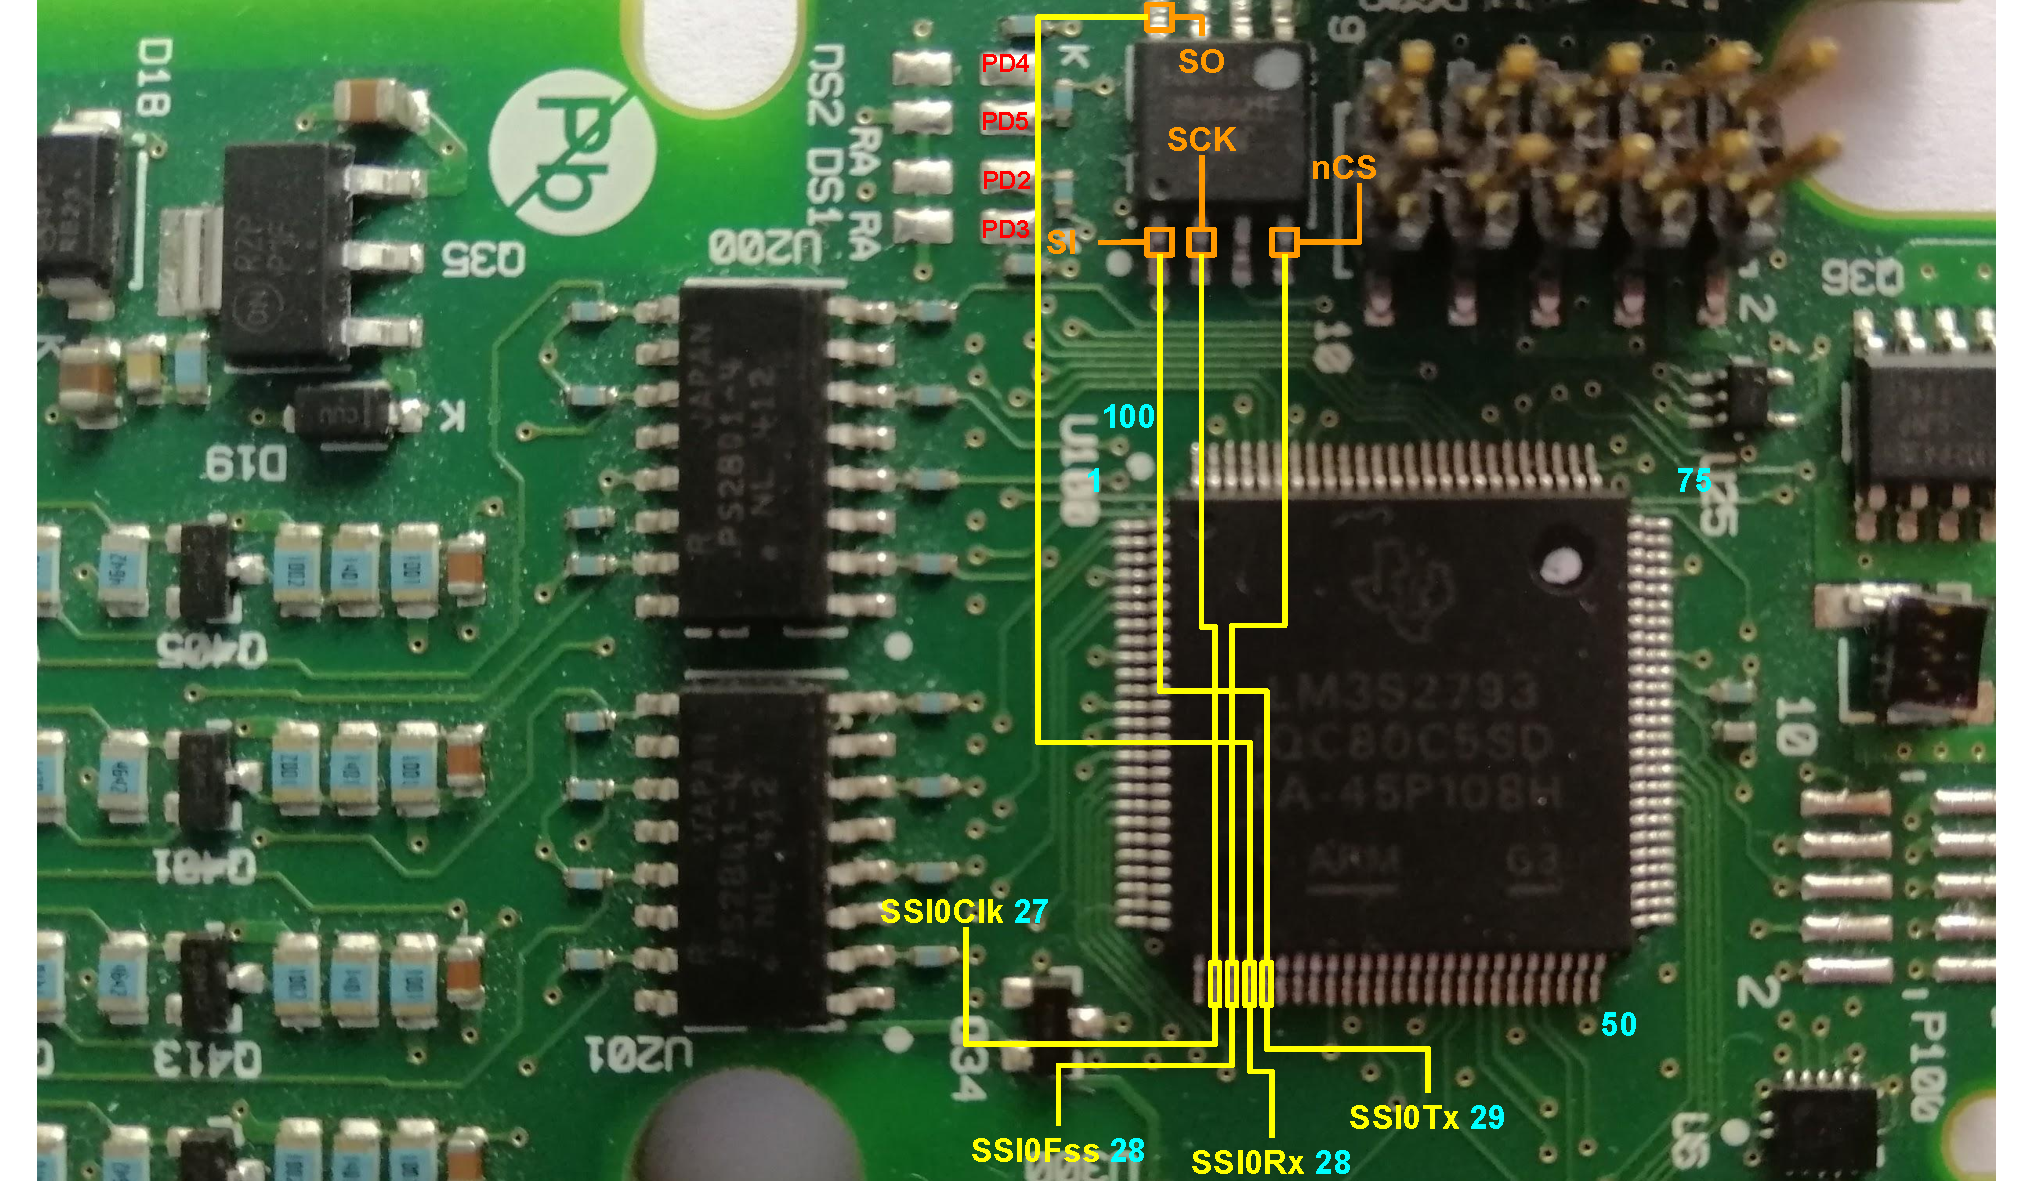
\includegraphics[width=0.47\textwidth]{figures/ssi0}
	\centering
	\caption{LM3S2793 SSI0 Pins Connect to AT45DB21E SPI Serial Flash Memory}
	\label{fig:ssi0}
\end{figure}

Also, at the beginning of the firmware initialization, right after copy part of the inner flash to RAM as we mentioned earlier, by associating GPIO port A and SSI0, the firmware first read a byte from the flash chip (at offset 0x2000). This byte is stored at address 0x20000F50. If the value of this byte is 0x55 or 0xAA, the firmware will reset the system, otherwise it will verify the firmware integrity from memory 0x4000 to 0x1FFFC. 

The checksum is very simple. From 0x4000 to 0x1FFFC, accumulate each byte, and the final result is compared with the byte at 0x1FFFF. If they are equal, the check passes, otherwise, the firmware enters an infinite loop and keeps reset the watchdog.

We can see that the variables saved in the external flash may indicate the state of the system's last run. Value 0x55 indicates something fatal happened. Right before it reset the system, the firmware setups 4 pins of GPIO port D as output and operates on it. We traced these 4 pins to a solder joint pad, as shown in~\autoref{fig:ssi0}, although this part is not installed.

Value 0xAA indicates that the firmware from 0x4000 to 0x1FFFF is corrupted. The firmware reloads the partial image from external flash chip (from offset 0x6100) and sets variable 0x20000F50 to 0, then resets the PLC. But this image from AT45DB021E is a default backup.


\subsubsection{Front Panel LED}

There are four rows of LED lights on the front panel, and each two rows (8 LEDs in each row) indicates the status of the input and output ports. Under the plastic case, the LEDs are mounted on the module E, as shown in~\autoref{fig:modules}. Those LEDs is a intuitive representation of the current PLC status.

There are two 24-pin chips also mounted on module E. Top-side marking says "PD9535". They are "Remote 16-bit I2C and SMBus, Low-Power I/O Expander"~\cite{pd9535}. It provides general-purpose remote I/O expansion for most microcontroller families via the I2C interface, SCL (serial clock) and SDA (serial data). Combined with the reverse engineering of the firmware, it can be determined that the two chips are connected to the microcontroller on the module B through I2C protocol. I2C is a serial protocol for two-wire interface to connect low-speed devices like microcontroller, EEPROM, A/D and D/A converters, I/O interface and other similar peripherals in the embedded systems~\cite{semiconductors2000i2c}.

The module C and E are connected by module D through a proprietary interface. LM3S2793 uses two pins of GPIO Port B (PB2 and PB3) for peripheral I2C0 as the SCL and SDA. PB2/I2C0SCL and PB3/I2C0SDA correspond to pin 5 and pin 6 in of the  proprietary interface, as shown in~\autoref{fig:p607}.

Each I2C slave device has a 7-bit address that needs to be unique on the bus. Some devices have fixed I2C address while others have few address lines which determin lower bits of the I2C devices on the bus with unique I2C address. For PD9535, three hardware pins are used to program and vary the fixed I2C address and allow up to eight devices to share the same bus. In our case, the addresses of thses two PD9535 slave devices on module E are 0x20 and 0x21 respectively. More specifically, 0x20 corresponds to the 16 LED lights of the input ports, 0x21 corresponds to the other 16 LED lights of the output ports. 

The PD9535 consists of two configuration, input port, output port and polarity inversion registers, each register has 8 bits. The master device can enable the I/Os as either inputs or output port by writing to the configuration port.

I2C communication begins with a master device sending a start condition which is a high-to-low transition on the SDA while the SCL is high. After the start condition, the slave device address byte is sent, most significant bit first. The first 7 bits are the slave address, and the last bit of the byte is the data direction bit, 1 indicates reading, 0 indicates writing. Only the slave device the specific address will respond to this transmission and acknowledge the byte by pulling a low on the SDA during a SCL pulse. Following the successful acknowledgement of the address byte, the master device sends a command byte that is stored in the control register. Only the lowest 3 bits are used to state the operation and aforementioned 8 registers will be changed accordingly. The command byte is shown in the following table.

\begin{center}
	\begin{table}
		\begin{tabular}{|c|c|c|} 
			\hline
			\makecell{COMMAND \\BYTE} & REGISTER & OPERATION \\ [0.5ex] 
			\hline
			0x00 & Input Port 0 & Read \\ 
			\hline
			0x01 & Input Port 1 & Read \\
			\hline
			0x02 & Output Port 0 & Read/Write \\
			\hline
			0x03 & Output Port 1 & Read/Write \\
			\hline
			0x04 & Polarity Inversion Port 0 & Read/Write \\
			\hline
			0x05 & Polarity Inversion Port 1 & Read/Write \\
			\hline
			0x06 & Configuration Port 0 & Read/Write \\
			\hline
			0x07 & Configuration Port 1 & Read/Write \\
			\hline
		\end{tabular}
		\caption{Control Register Command Byte}
		\label{tab:i2ccommand}
	\end{table}
\end{center}


The following pseudo code uses aforementioned ROM API to initialize the I2C slave device for the output port LED lights.

\begin{lstlisting}[style=code, caption={Pseud Code for Initializing the I2C Slave Device for the Ouput Port LED Lights}, captionpos=b]
ROM_SysCtlPeripheralEnable(SYSCTL_PERIPH_I2C0);
ROM_GPIOPinTypeI2C(0x40059000, 0xC);
clock = ROM_sysCtlClockGet();
ROM_I2CMasterInitExpClk(0x40020000, clock, TRUE);
ROM_I2CMasterSlaveAddrSet(I2C0, 0x21, FALSE);
ROM_I2CMasterDataPut(I2C0, 0x6);
ROM_I2CMasterControl(I2C0, I2C_MASTER_CMD_BURST_SEND_START);
while (ROM_I2CMasterBusy(I2C0)) {
};
ROM_I2CMasterDataPut(I2C0, 0x0);
ROM_I2CMasterControl(I2C0, I2C_MASTER_CMD_BURST_SEND_COUNT);
while (ROM_I2CMasterBusy(I2C0)) {
};
ROM_I2CMasterDataPut(I2C0, 0x0);
ROM_I2CMasterControl(I2C0, I2C_MASTER_CMD_BURST_SEND_FINISH);
while (ROM_I2CMasterBusy(I2C0)) {
};
\end{lstlisting}

After initialization, the following code shows how to control the 8 LEDs corresponding to the output port by sending a byte to Output Port 0. We send 0xFF, which means that 8 LEDs are lit.
\begin{lstlisting}[style=code, caption={Pseud Code for Controlling LED Lights}, captionpos=b]
ROM_I2CMasterDataPut(I2C0, 0x2);
ROM_I2CMasterControl(I2C0, I2C_MASTER_CMD_BURST_SEND_START);
while (ROM_I2CMasterBusy(I2C0)) {
};
ROM_I2CMasterDataPut(I2C0, 0xFF);
ROM_I2CMasterControl(I2C0, I2C_MASTER_CMD_BURST_SEND_COUNT);
while (ROM_I2CMasterBusy(I2C0)) {
};
\end{lstlisting}


\subsubsection{Connections Between Modules}

To answer the question who update the compiled ladder logic code to the real-time microcontroller, we need to further know about how the module are connected. Of all the connectors, the one connecting module B and module C is the most important, as shown in~\autoref{fig:board}. 

\begin{figure}[th]
	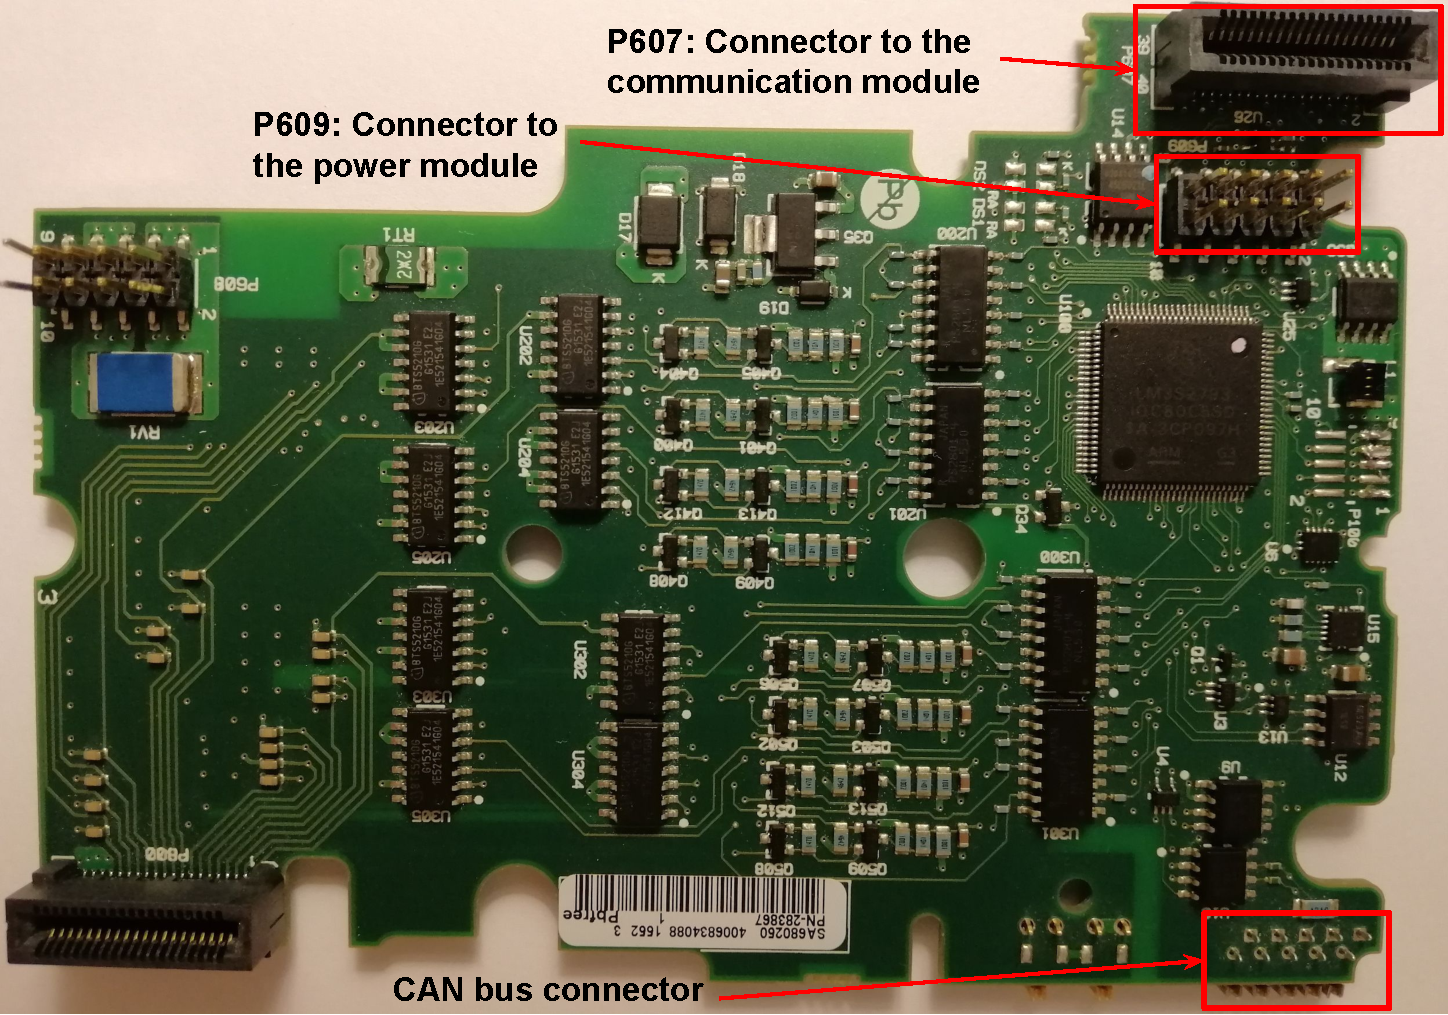
\includegraphics[width=0.47\textwidth]{figures/board}
	\centering
	\caption{The Real-time Module}
	\label{fig:board}
\end{figure}

Because the communication module B is responsible for communicating with SCADA system and transmitting new data to the real-time module C in a timely manner. With some reverse engineering effort, we figured out the function of most of the pins of this proprietary interface, as shown in~\autoref{fig:p607}.

\begin{figure}[th]
	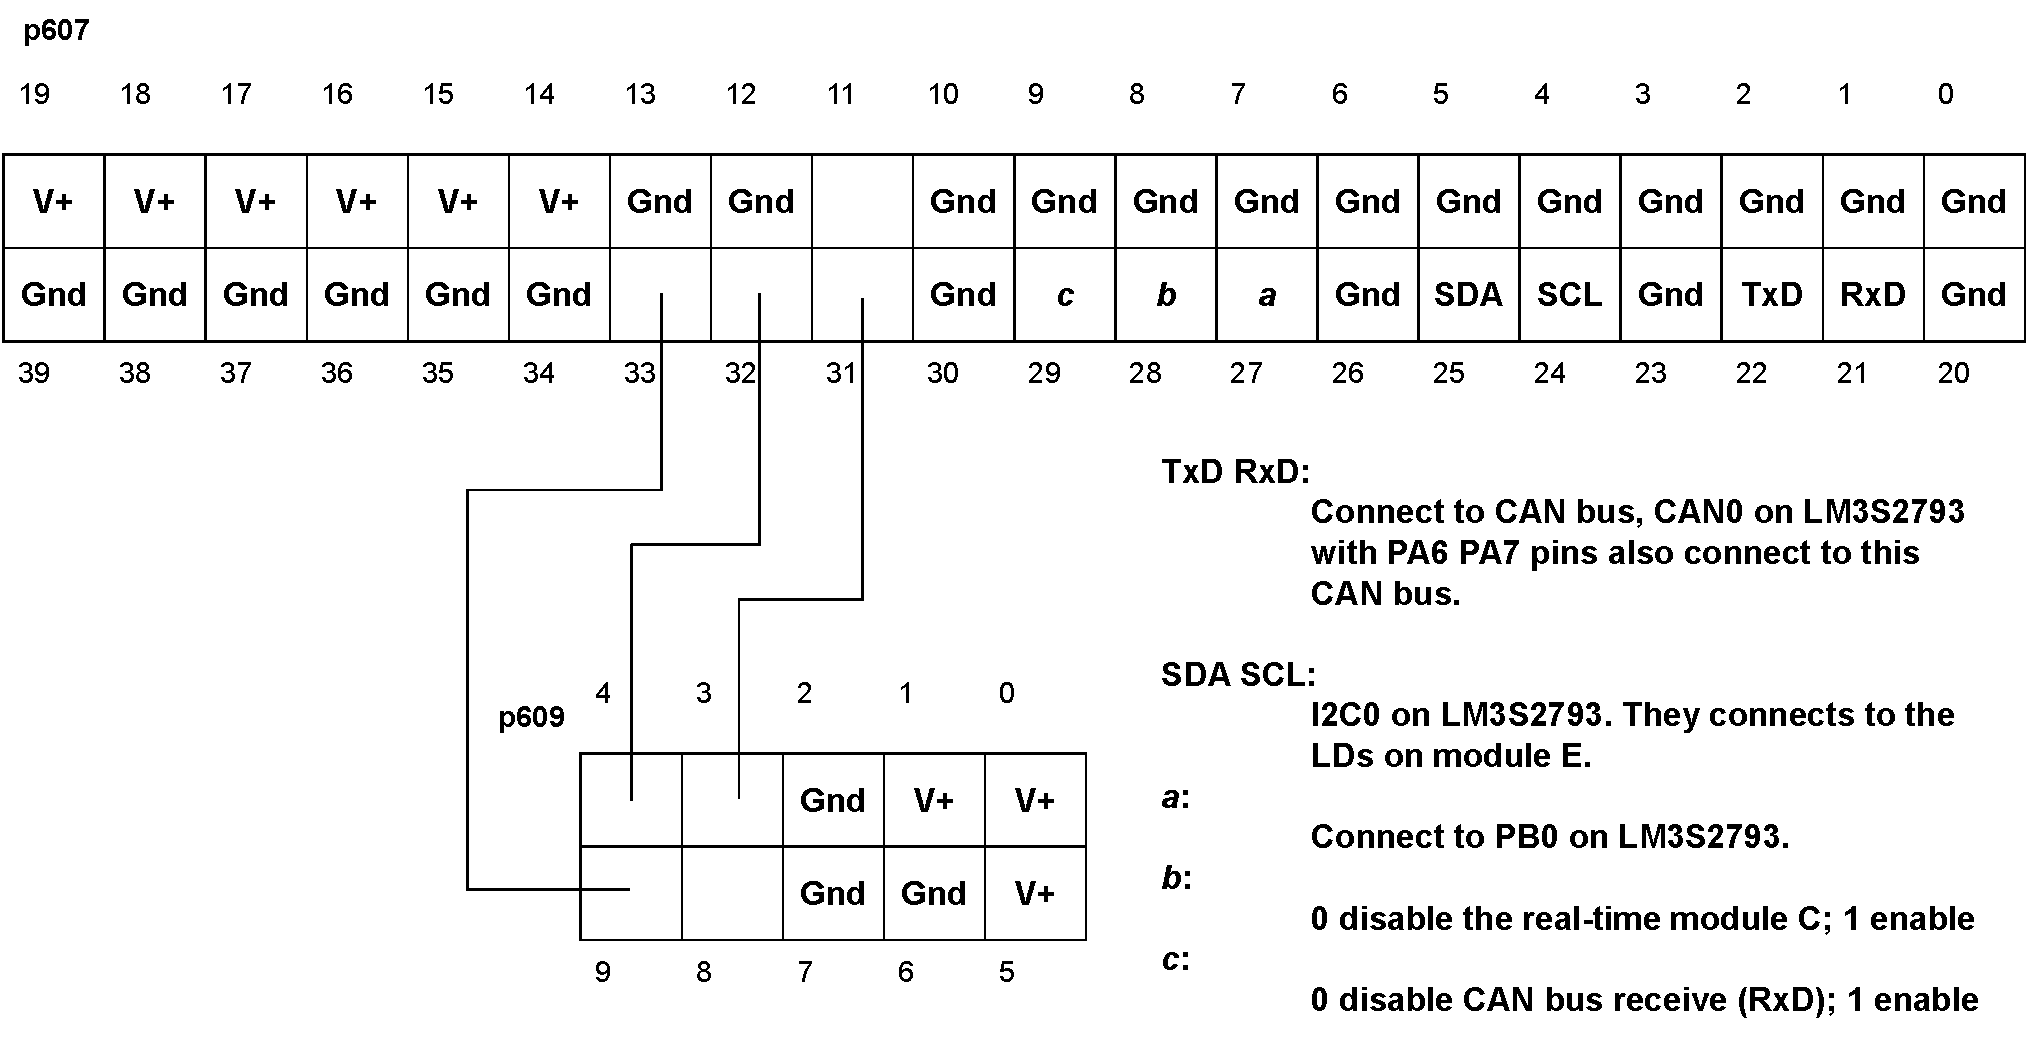
\includegraphics[width=0.47\textwidth]{figures/p607}
	\centering
	\caption{Connector between Module B and Module C (p607)}
	\label{fig:p607}
\end{figure}

As mentioned earlier, on module C, there is a AT45DB21E flash chip. It connects to the microcontroller through SSI0. And it contains one copy of code that will be loaded in once the microcontroller is caught in an unrecoverable error. But by analyzing this interface, we found that the communication module B is not connected to this AT45DB21E flash chip. So we think the code in it is just the backup code used to recover from the fatal error state, and the updated compiled ladder logic is updated by other means.  

By reverse engineering the circuit board and firmware, we identified pin 24 and pin 25 of the connector as the SCL and SDA pin of I2C bus, as shown in~\autoref{fig:p607}. The microcontroller LM3S2793's PAxx PAxx connects LED module E through the communication module B, as shown in~\autoref{fig:modules}.

We also identified that pin 21 and pin 22 are used as CAN bus input and output that come from the communication module B. And pin 29 is used to disable the CAN bus receive signal (RxD). On the CompactLogix PLC 1766, there is only one set of CAN bus for connecting modules. It located on the side of the PLC, it's part of the real-time module, as shown in~\autoref{fig:board}.


Both the communication module B and real-time module C are connected to this bus.

